\chapter{基于图过滤的程序依赖图表征学习}
\label{chap:PDG}
本章主要对本文提出的基于图过滤的程序依赖图表征学习方法进行详细介绍,首先介绍其基本思想,其次阐述其具体方法设计与实现,最后进行实验验证。

\section{研究动机}
\label{sec:PDGMotivation}

程序依赖图PDG是代码的一种图形表示,所含结构信息最多,能够表示程序的控制依赖,数据依赖等关系,是一种带有标记的有向多重图。程序依赖图PDG结点代表语句,边代表依赖关系,依赖关系包括数据依赖和控制依赖。基于图的代码表征方法首先使用代码分析工具构建包含代码语法结构、调用关系、数据流等信息的程序依赖图,然后通过图匹配的方法,将PDG图中的控制流和数据流编码为一个紧凑的语义特征矩阵,其中每个元素都是一个高维的稀疏二值特征向量,通过寻找矩阵之间的相似模式来判定克隆代码。通过将代码表示为图的形式使得模型能够更好地理解代码中不同部分之间的依赖关系。

基于图的代码表征方法存在两种主要限制:

(1)复杂度较高:基于图的代码克隆检测方法通常需要构建代码的结构图或控制流图,然后对这些图进行比较。这个过程可能涉及复杂的图算法,导致计算成本较高,尤其是在处理大规模代码库时。难以处理复杂结构:对于具有复杂控制流或数据流的代码,构建准确的图表示可能是一个挑战。此外,对于具有循环、递归或异常处理的代码,图的构建和比较可能更加困难

对代码修改的敏感性:当代码发生小的修改时(例如变量名更改、代码格式化、添加或删除注释等),这些修改可能会导致图的表示发生显著变化。因此,基于图的克隆检测方法可能无法准确地检测出这些轻微修改过的克隆代码。
可扩展性和可维护性:随着代码库的不断增长和变化,基于图的克隆检测方法可能需要不断地更新和调整以适应新的代码结构。这可能导致维护成本较高,并且难以保证方法的长期有效性。






\section{PDG表征方法方法设计}
\label{sec:PDG}
本节将介绍基于图过滤的程序依赖图表征学习方法设计与实现,首先介绍该方法的整体框架,并从图过滤、程旭依赖图表征学习两方面介绍具体设计。 

\subsection{框架概述}
\label{subsec:PDGOverview}
本文提出的基于图过滤的程序依赖图表征学习方法整体框架如图\ref{fig:pdgframework}所示。该框架的输入是代码片段对应的程序依赖图,输出是对应的语义特征向量,主要包括图过滤、图表征两个阶段。

\begin{figure}[H]
  \centering
  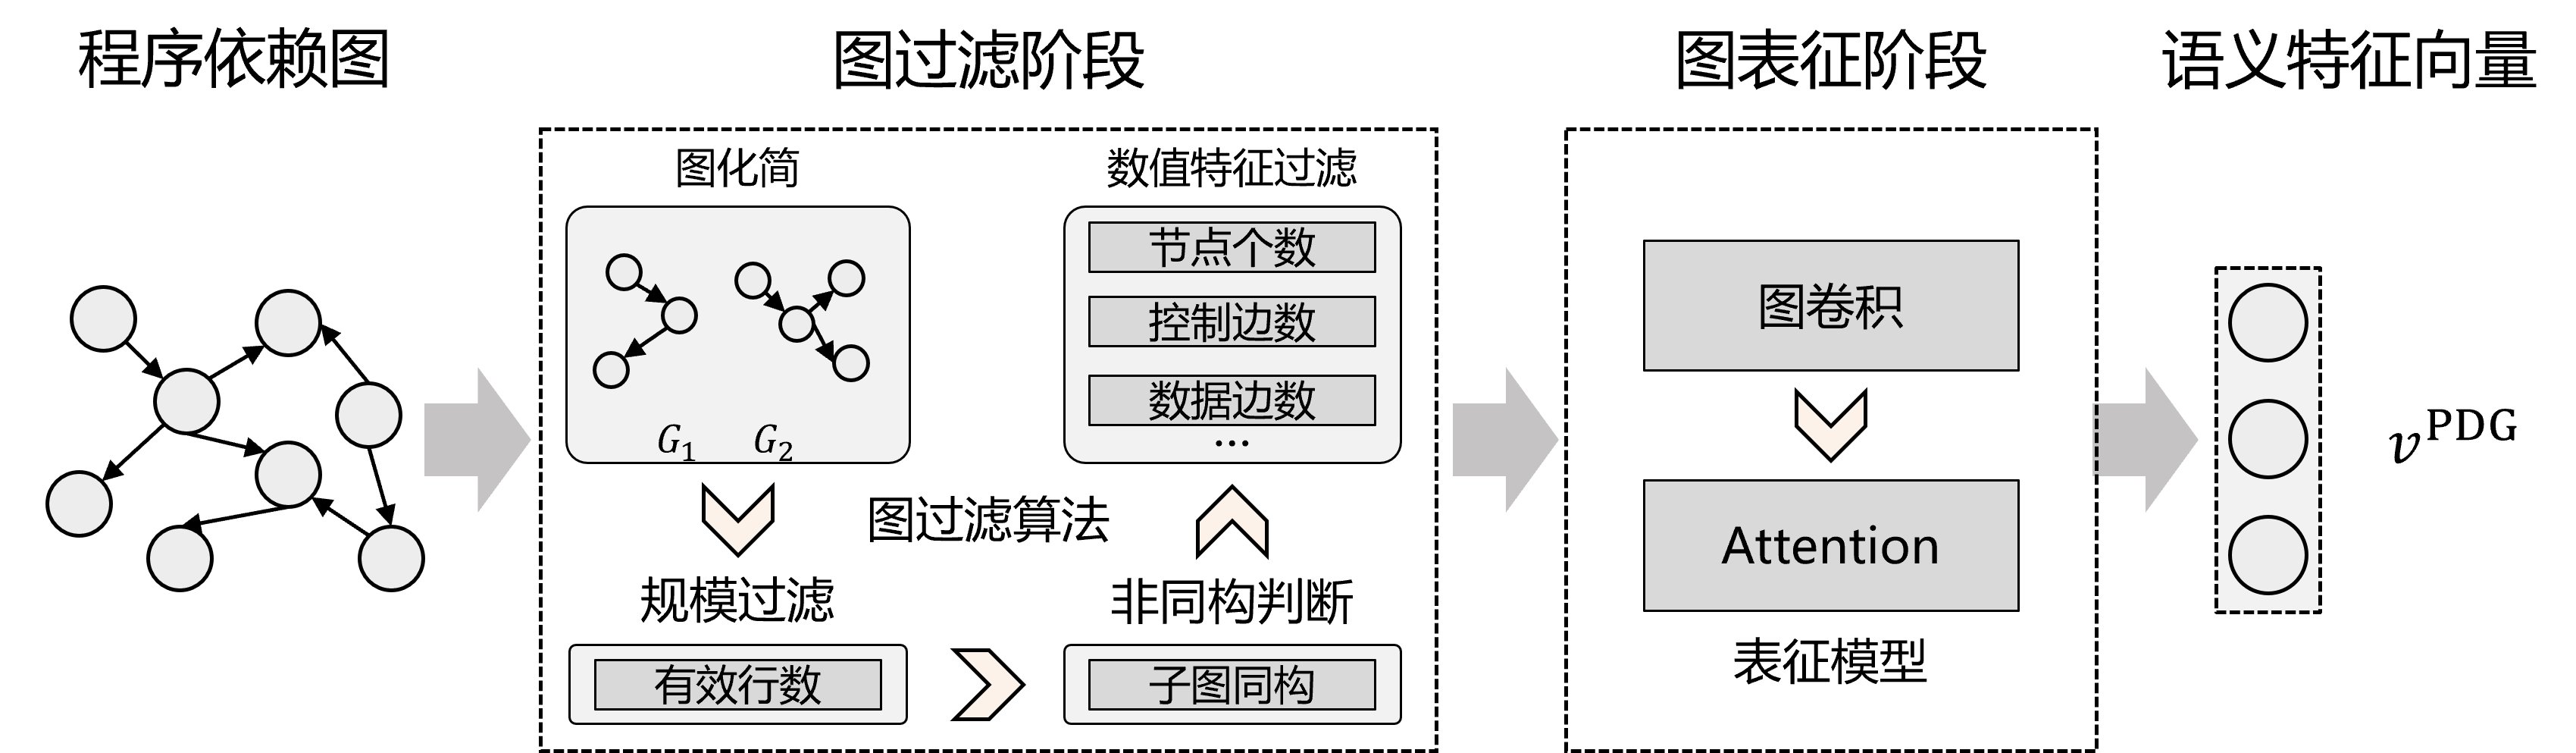
\includegraphics[width=0.95\textwidth]{figures/pdgframework.png}
  \caption{基于图过滤的程旭依赖图表征学习框架}\label{fig:pdgframework}
\end{figure}

首先,

其次,

在上述框架中,


\subsection{图过滤设计}
\label{subsec:PDGPreModel}

基于图的代码克隆检测方法需要将生成的程序依赖图两两匹配,对于包含$n$个代码片段的数据集,需要进行$n_2$次匹配检测,而其中包含大量无用的匹配,会浪费大量的时间和计算资源。


针对上述问题,本文引入一种图过滤算法,



通过收集PDG的简单特征来过滤掉明显不可能为克隆的PDG对。具体的,根据PDG的节点个数、控制边数、执行边数、数据边数、声明节点数、函数调用数、传入参数、传出参数等代表特征进行过滤,在大幅减少候选PDG对规模的同时,保证真正的克隆对不会被过滤掉而导致整体克隆检出率的降低。

是代码PDG G的特征向量。Pf是代码PDG-Gf的特征向量,L是PDG中节点数的阈值,T是PDG对的尺度无线电的阈值。GN是特征向量的数值相似度的阈值

\begin{algorithm}[ht]  
	\renewcommand{\algorithmicrequire}{\textbf{Input:}}
	\renewcommand{\algorithmicensure}{\textbf{Output:}}
	\caption{Graph filter algorithm $\left(filter\_PDG\right)$}  
	\label{alg3}
	\begin{algorithmic}[1]
    \Require PDG pairs:$G$
    \Require The threshold:$L$
    \Require The threshold:$T$
    \Require The threshold:$G_s$
		\Ensure Candidate PDG pairs:$R$
    \State initialization
		\For{each PDG paris $G_1,G_2$  $in$ $G$}
      \If {sizeof($G_1$) < sizeof($G_2$) < L}
        \State PDG pair($G_1,G_2$) is filtered
      \Else
        \If {min($G_1,G_2$) / max($G_1,G_2$) < T}
          \If{there is subgraph between ($G_1,G_2$ )}
            \State R $\leftarrow$ R $\cup \left(G_1,G_2\right)$
          \Else
            \State PDG pair($G_1,G_2$ ) is filtered
          \EndIf
        \Else
          \If {number similarity of $G_1,G_2$ > $G_s$} 
            \State R $\leftarrow$ R $\cup \left(G_1,G_2\right)$
          \Else
            \State PDG pair($G_1,G_2$ ) is filtered
          \EndIf
        \EndIf
      \EndIf 
    \EndFor \\
    \Return $R$
	\end{algorithmic}
\end{algorithm}

\subsection{程序依赖图表征学习设计}
\label{subsec:PDGModel}

(1)结构设计

为了提高程序依赖图维度代码表征能力,本文选取图卷积网络对上述得到程序依赖图进行建模。具体的模型设计如图\ref{fig:pdgmodel}所示。该模型主要包括输入层、多层卷积层、自注意力层、输出层。
\begin{figure}[H]
  \centering
  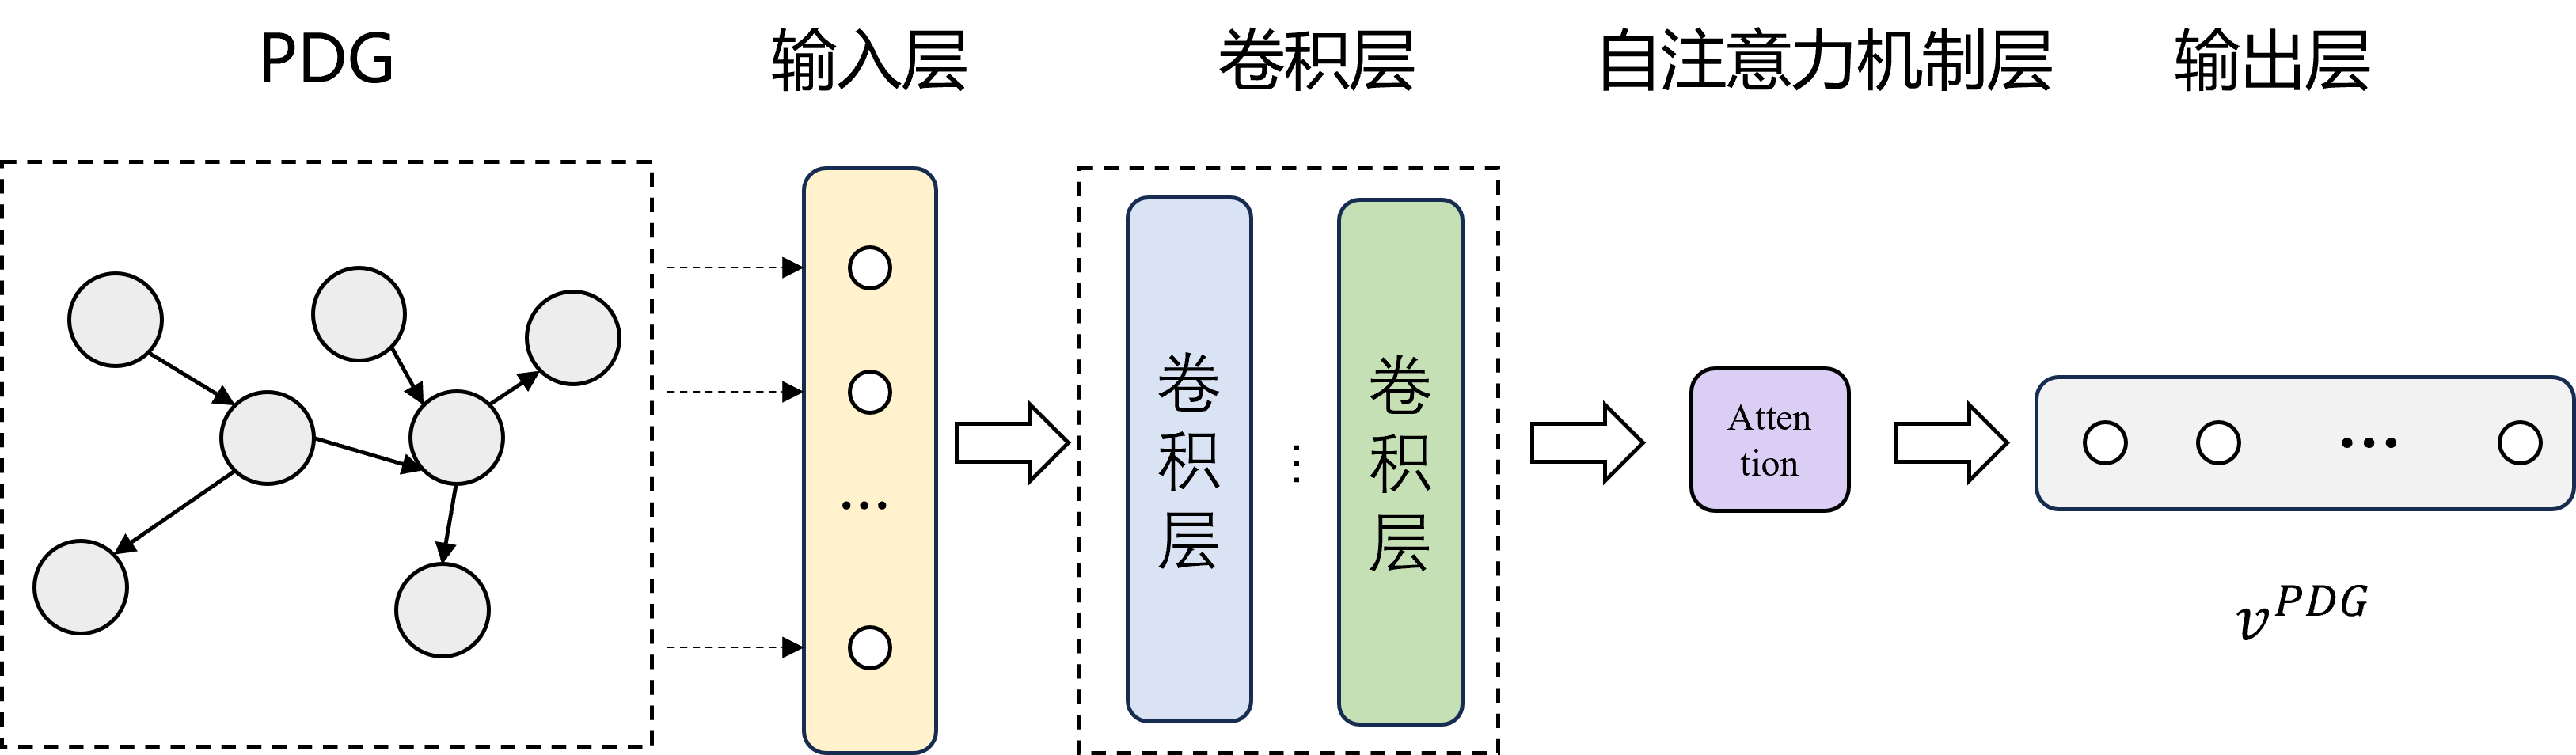
\includegraphics[width=0.85\textwidth]{figures/pdgmodel.png}
  \caption{程序依赖图表征模型设计}\label{fig:pdgmodel}
\end{figure}

(2)模型选型


对于提取到的程序依赖图,本课题拟通过图卷积神经网络将其转换成向量。


图卷积神经网络是一种特殊的前馈神经网络结构,为减少网络中参数个数,用卷积层来代替传统的全连接层,提高神经网络的训练效率,卷积神经网络可以提取信息最多的数据特征,生成一个固定大小的向量表示结构,从而挖掘深层次的语法和语义信息,在代码克隆检测任务中有较好的性能表现。

图卷积神经网络(GCN)的基本原理是通过卷积操作来提取图中节点的特征信息。在GCN中,节点的特征表示会考虑其邻居节点的特征,并通过学习得到的参数来更新。通过多层GCN的堆叠,可以逐步传播全局信息,实现对整个图的信息聚合和表示学习。GCN特别适合于那些节点表示和节点间关系都很重要的问题,如社交网络分析、分子结构识别、推荐系统等。


图中的每个结点无时无刻不因为邻居和更远的点的影响而在改变着自己的状态直到最终的平衡,关系越亲近的邻居影响越大。

GCN的主要思想:对于每个结点,我们都要考虑其所有邻居以及其自身所包含的特征信息。假设我们使用average()函数,那对每一个结点进行上述操作后,就可以得到能够输入到神经网络的平均值表示。



\section{PDG表征方法具体实现}
\label{sec:PDGachieve}
在介绍具体实现之前,本节首先给出PDG表征方法的输入:经过\ref{subsec:Preprocess}小节的代码预处理阶段,得到示例代码片段\ref{fig:code}对应的程序依赖图,如图\ref{fig:pdgcode}所示。图中的实线表示节点之间的控制依赖,虚线表示节点之间的数据依赖。仔细分析三张图,其中图\ref{fig:pdg1}和图\ref{fig:pdg2}红框中节点11、12虽然位置有所改变,但是其边依赖均相同,因此可以视为完全相同的同构图;而图\ref{fig:pdg3}因为增加了一个if语句,图中也增加了一个节点,同时添加的红色的线表示新增的数据依赖、控制依赖。

\begin{figure}[htbp]
  \centering  %居中
  \subfigure[C语言代码片段1对应的PDG]{   %第一张子图
      \centering    %子图居中
      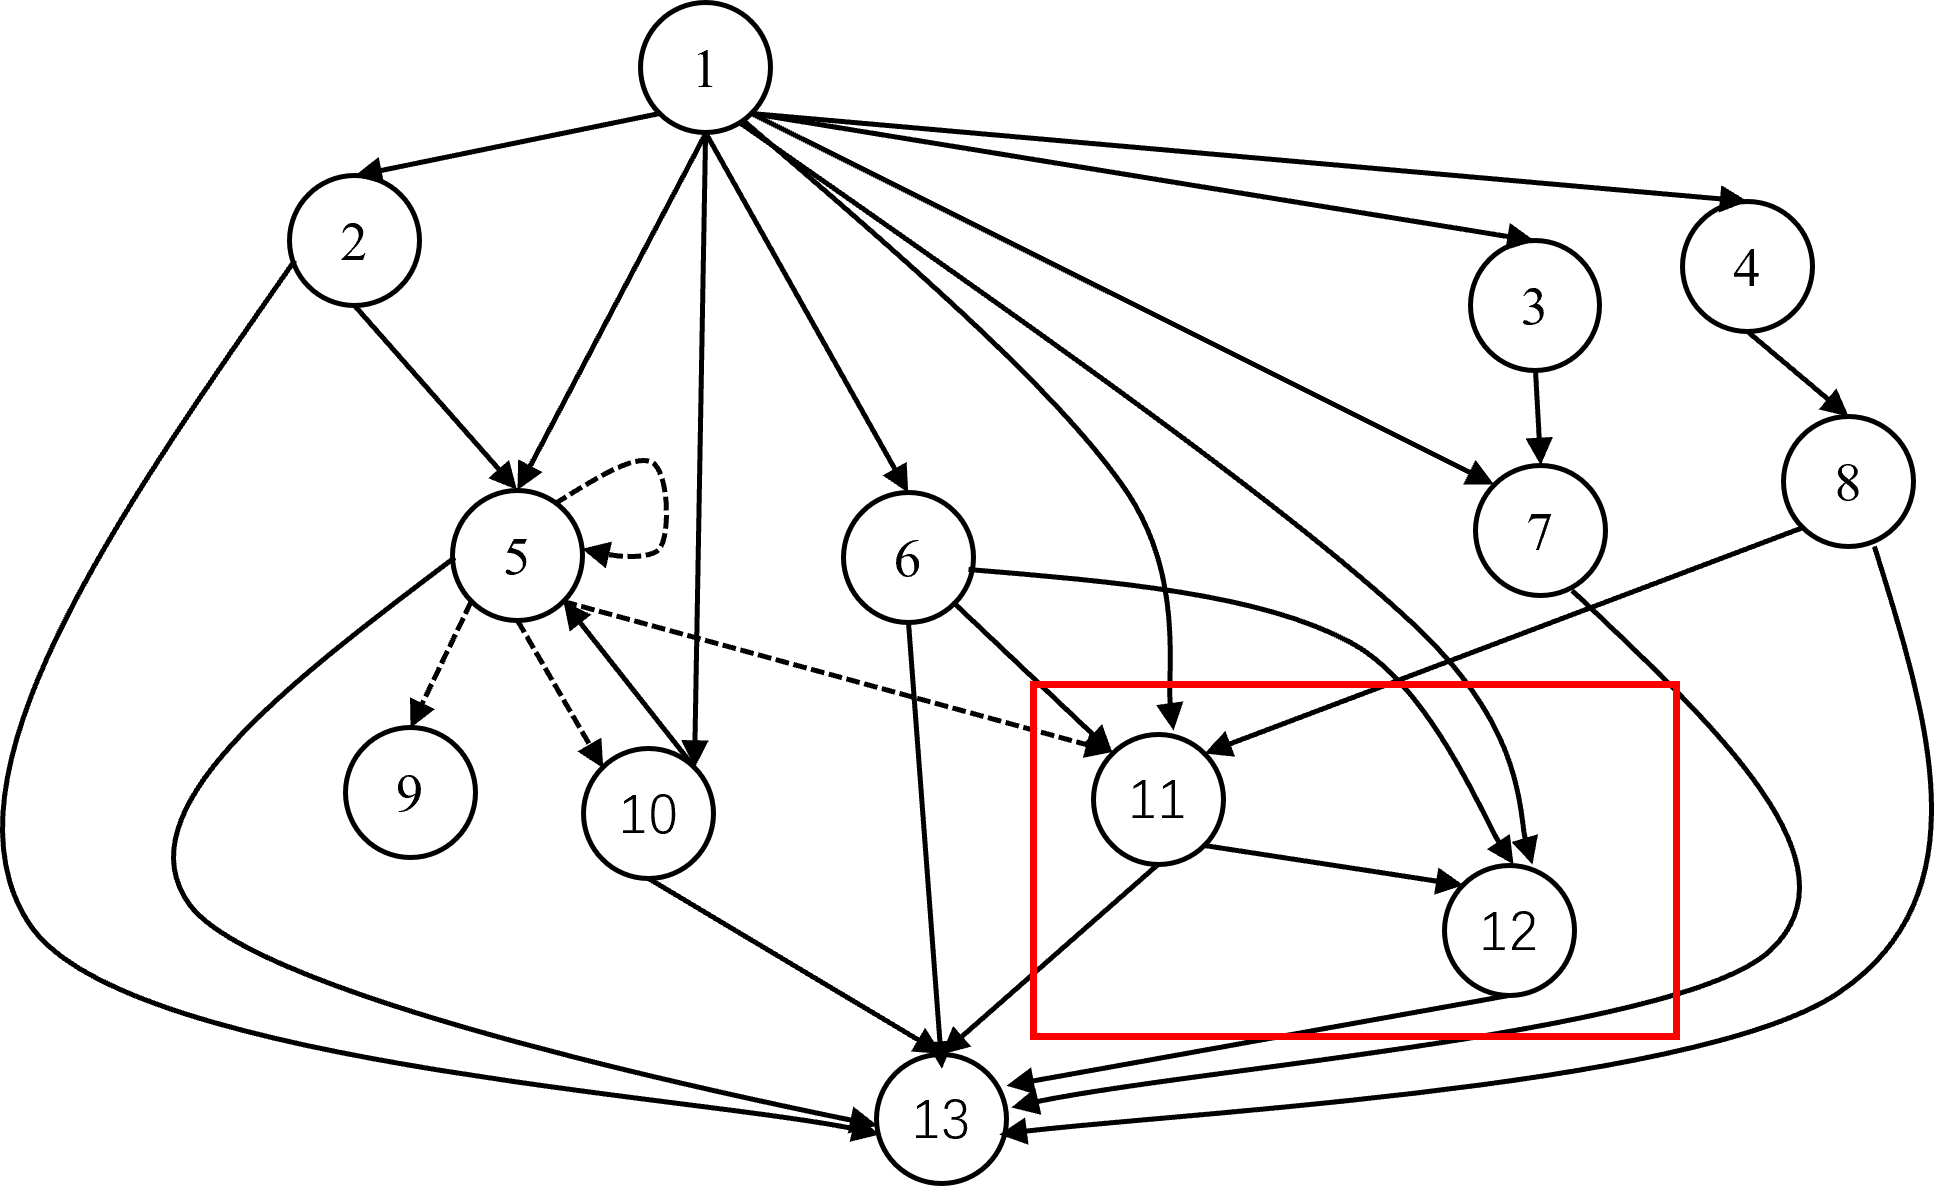
\includegraphics[width=0.3\textwidth]{figures/pdg1}  
      \label{fig:pdg1} %引用标签
  }
  \subfigure[C语言代码片段2对应的PDG]{ %第二张子图
      \centering    %子图居中
      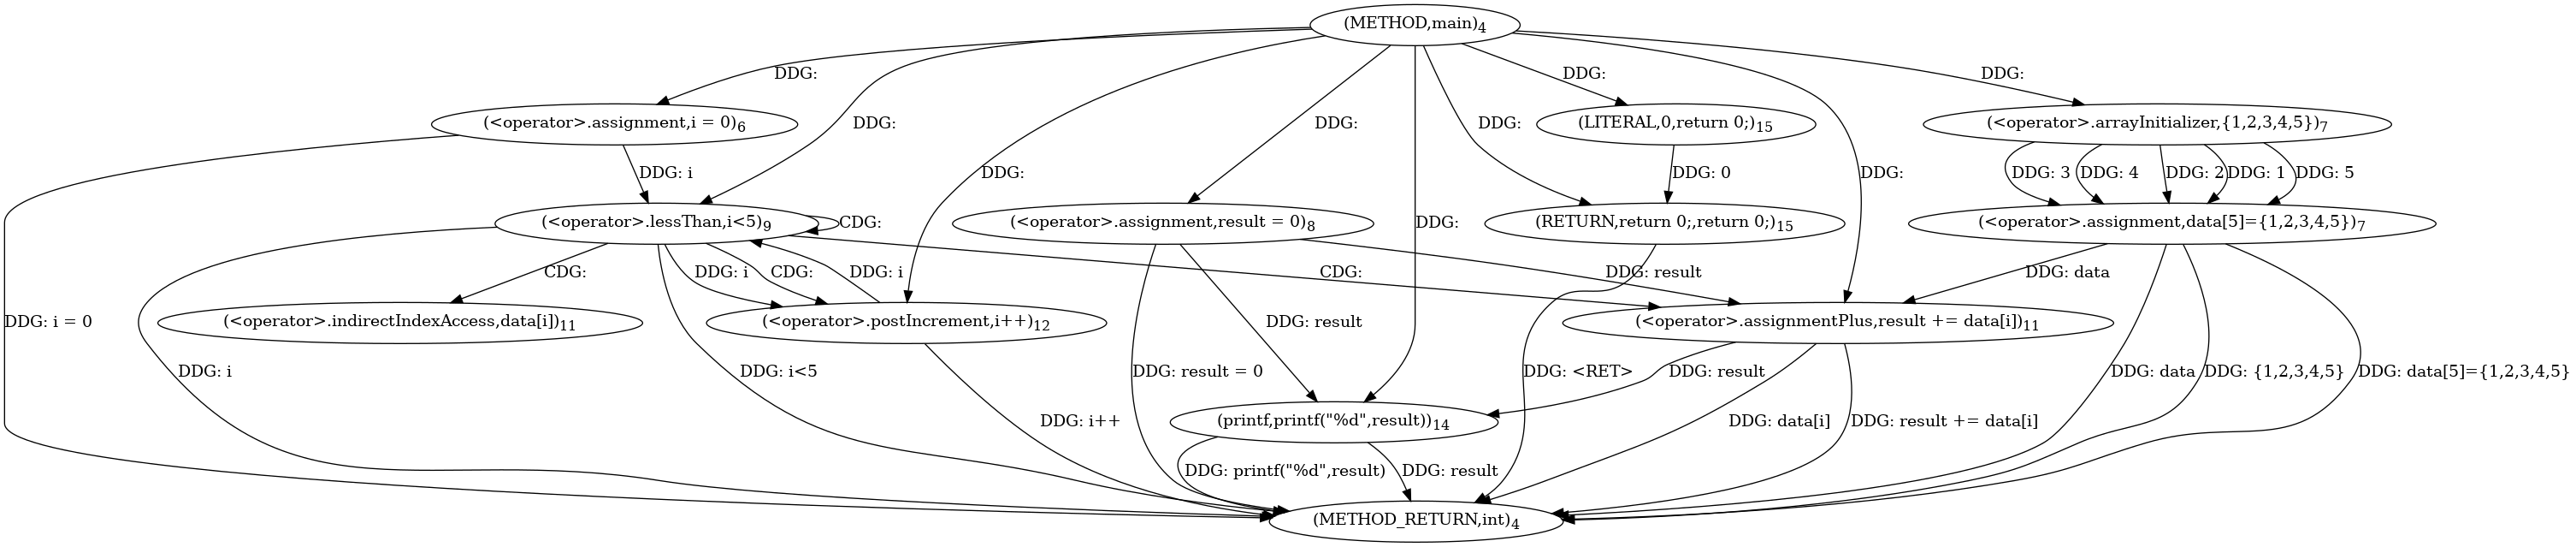
\includegraphics[width=0.3\textwidth]{figures/pdg2}
      \label{fig:pdg2} %引用标签
  }\subfigure[C语言代码片段3对应的PDG]{ %第二张子图
  \centering    %子图居中
  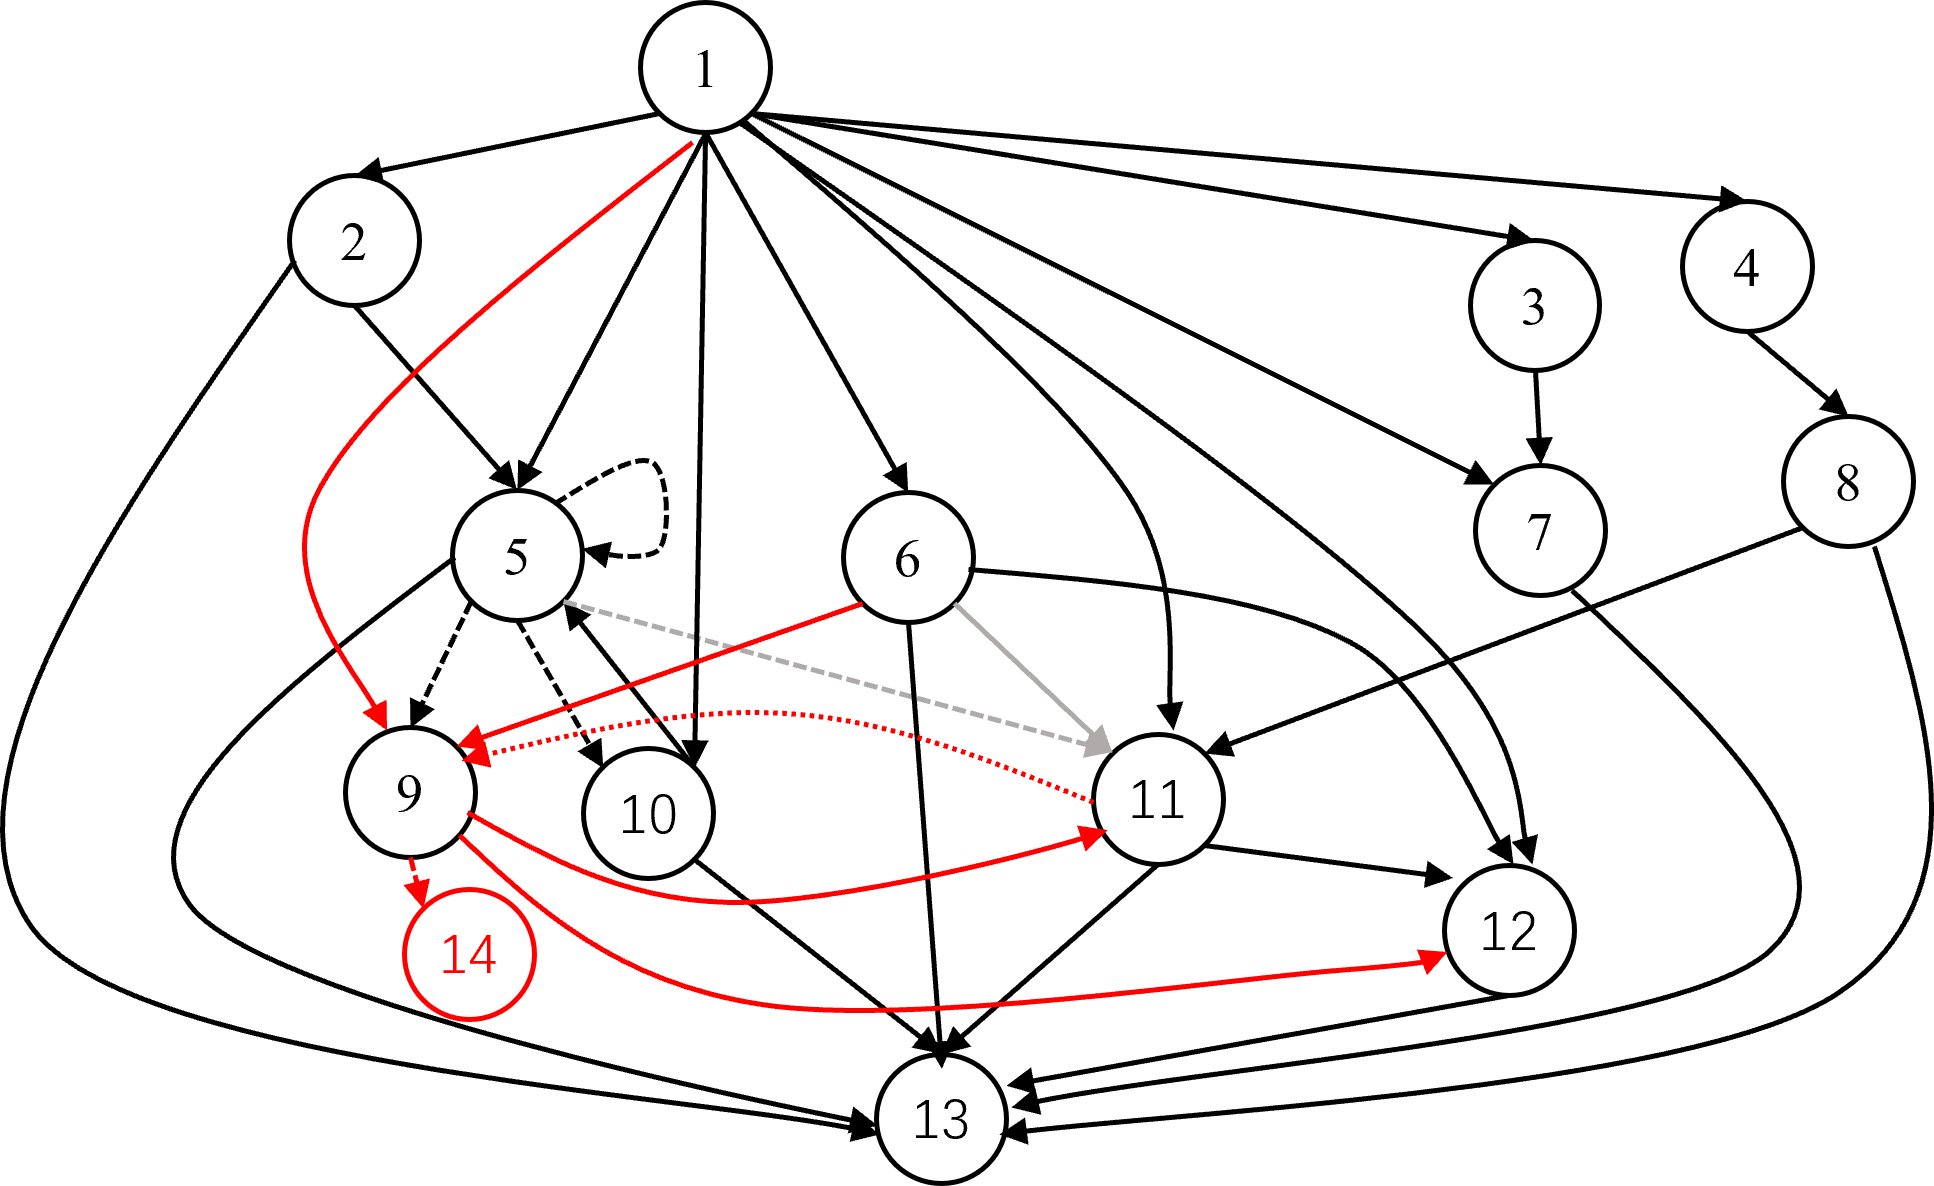
\includegraphics[width=0.3\textwidth]{figures/pdg3}
  \label{fig:pdg3} %引用标签
}
  \caption{示例源代码对应的程序依赖图}    %大图名称
  \label{fig:pdgcode}    %图片引用标记
\end{figure}

接下来,本章提出的基于图过滤的程序依赖图表征学习方法的实现如图\ref{fig:pdg}所示。该方法的输入是一对代码片段$C_{a},C_{b}$对应的程序依赖图,表示为$PDG_{a},PDG_{b}$,输出是$C_{a},C_{b}$对应的语义特征向量 $V_{a}^{PDG},V_{b}^{PDG}$,整体采用Siamese架构,两个子网络共享权值,从下到上,主要包括图过滤判断、图表征三个阶段。

\begin{figure}[H]
  \centering
  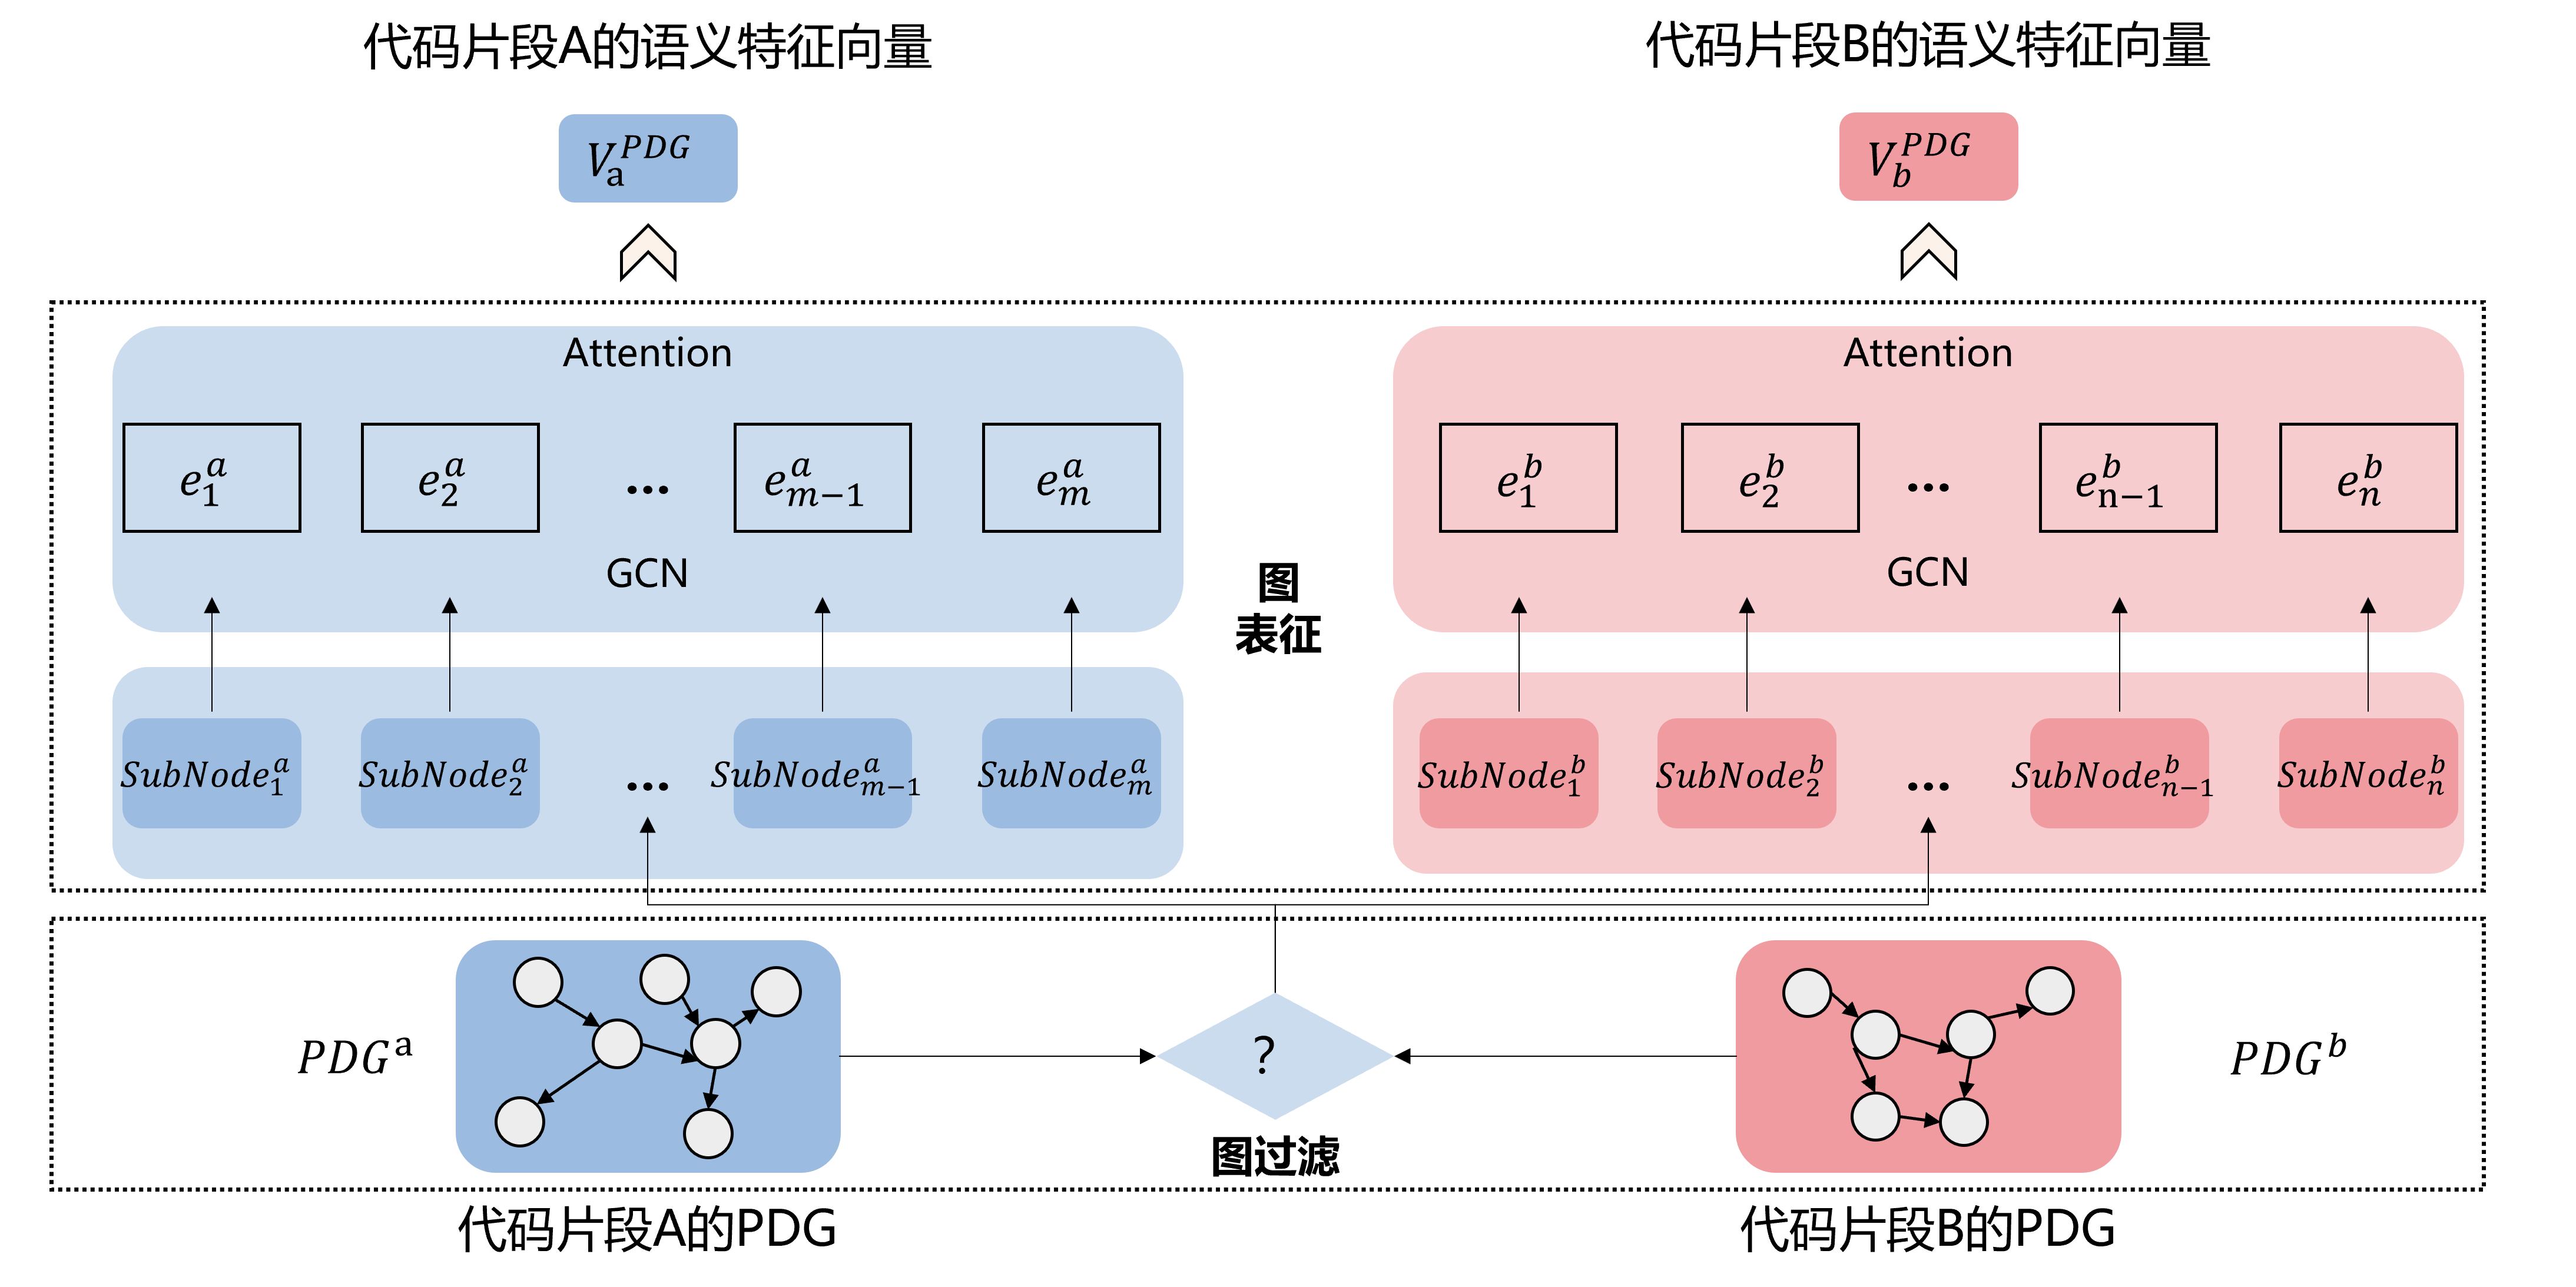
\includegraphics[width=0.9\textwidth]{figures/pdg.png}
  \caption{基于图过滤的程序依赖图表征学习方法实现}\label{fig:pdg}
\end{figure}

在图过滤阶段,

\section{实验验证}
\label{sec:PDGExperiment}
为了验证基于图过滤的程序依赖图表征学习方法的有效性,本文
\subsection{实验设计}
\label{sec:PDGDesign}
和3.3.1 相同
\subsection{实验结果}
\label{subsec:PDGResult}
消融对比实验:体现图过滤机制的有效性

基于PDG的GCN

基于PDG的+图过滤的GCN


\begin{table}
  \centering
  \caption{图过滤机制实验结果} %{tab:category}
  \begin{tabular*}{0.9\textwidth}{@{\extracolsep{\fill}}cccc}
  \toprule
    对比			&P		&R		&F1 \\
  \midrule
    基于PDG的GCN			&0.xx	&0.xx		&0.xx \\
    基于PDG的+图过滤的GCN			&0.xx		&0.xx		&0.xx \\
  \bottomrule
  \end{tabular*}
\end{table}

\section{本章小结}
\label{sec:Summary5}
本章主要对RLCCD中基于图过滤的程序依赖图表征学习方法的设计与实现进行详细阐述。首先介绍了程序依赖图维度的研究动机,其次介绍了程序依赖图表征学习的方法设计,具体论述了其整体框架、图过滤、图表征学习,接着开展实验验证,结果表明了此方法的有效性和模型的准确性。



